\documentclass[conference]{IEEEtran}
\usepackage{blindtext, graphicx, url}
\graphicspath{ {images/} }
\ifCLASSINFOpdf
  
\else
  
\fi

\hyphenation{op-tical net-works semi-conduc-tor}


\begin{document}

\title{Energy Effecient Encryption in Wireless Sensor Network}


\author{\IEEEauthorblockN{Vipul Gupta}
\IEEEauthorblockA{Electronics and\\Communication Engineering\\
Indian Institute of Technology Roorkee\\
Roorkee-247667, Uttrakhand\\
Email: vipul26.h@gmail.com}
}

\maketitle


\begin{abstract}
%\boldmath
Wireless sensor networks(WSN) are being widely used and is one of the key areas of research. These devices are wearable and implantable. Body sensor networks play a major role in minimizing the needs of caregivers and provides people with quality care and reduces the chances of death in case of potentially harmful diseases. These devices are made based on various factors like unobtrusiveness, scalability, energy efficiency, security. This paper introduces the problems faced by WSN in fields of energy effeciency and security. One of the key part which we will discuss is related to public Key identification, it is one of the most effective way to establish secure connection between devices but in case of Wireless Sensors the energy consumed should be minimized so a different scheme should be proposed for encryption, as in public key generation and computation large processing power is utilised, so many different power effecient techniques are discussed and presented in this paper.
\end{abstract}

\begin{IEEEkeywords}
Wireless Sensor Network, Embedded system, AES Encryption, RC5 Encryption, ad hoc, Intrusion Detection Systems
\end{IEEEkeywords}

\IEEEpeerreviewmaketitle



\section{Introduction}
\begin{flushleft}
Wireless sensor networks(WSN) are being used in many fields like Area Monitoring, health care monitoring, environmental/earth sensing, industrial monitoring, etc. WSN is solving one of the most crucial problem of the world, that is health care problems which comes with old age. People have to spend lots of money to take the healthcare services and sometimes it is too late to provide the medicine to patient at the right time. To deal with all these problems wireless sensor networks can be used, a monitoring device can be connected through wireless network and if any abnormality is detected then it will send a signal telling the sensor to inject the medicine in the patient or will inform about the condition of patient \cite{WSNHM}. It is not only targeted to the elderly but can also help in providing quality services to the weak and fragile babies who don't have there parents watching over them for whole day due to work. These devices are wearable\cite{SWBS} and they can also be embedded inside the body.
\end{flushleft}
\begin{flushleft}
Currently the WSN is not much utilised because of the availability of old technology, which basically restricts our body in making any movements. Because of the ease of movement the WSN technology is being used widely. When these sensors are embedded inside the body, then the sensor becomes a part of network called Body Sensor Networks(BSN)\cite{HHMSWSN}. These devices help in monitoring, memory enhancement, control of home appliances, medical data access, and communication in emergency situations without restricting the movement of body.
\end{flushleft}
\begin{flushleft}
The sensors which are embedded inside the body are generally replacable(not rechargable due to infection concerns) and costs a lot, so they need to consume as less energy as possible. The general concerns involved in recharging are infection due to corrosion of rechargable metal, charging through radiation concerns, etc. So one of the way of reducing the health issue is creating a sensor which can be implantated inside the body and works for a long period of time. But creating Energy effecient devices like that is one of the issue that we are facing in the current scenario. There is trade off of energy and vulnerability, energy and health, energy and data transmission, etc. So in this paper we are going to take a look at one of the key factors that increase the energy consumption of the device, which is the use of many modern cryptographic algorithms to secure the communication between channels and prevent any malicious person to interfere with the patient's sensor device.As Wireless network is more vulnerable as compared to wire path like spoofing, packet change, parking lot attacks, etc, so to avoid all these attacks and to increase the energy effeciency, a lot of methods for encryption are being found out which uses the internal mechanism of the body or some other symmetric key algorithm to increase the device life. We know that reducing energy is always accompanied by increasing vulnerability while using cryptographic algorithm(reducing key size increases energy effeciency but also decreases security). And there are many conditions which must be met before using a particular algorithm in a particular condition so we will be looking into the usage of many algorithms which are being used in the sensor networks and also discussing about the drawback of using the asymmetric key encryption.
\end{flushleft}

\subsection{Working of Wireless Sensor Networks}
\begin{flushleft}
Wireless Sensor Networks consists of three main components called gateway, nodes and softwares. Wireless measurement systems can overcome power and network infrastructure limitations and deliver reduced costs and reliability as compared to wired connection. WSN nodes can vary from tens to hundreds to thousands, in which one node can be connected to one or several sensors. WSN node generally consists of several parts including radio transceiver with an internal or connection to an external antenna, also a microcontroller used to control the working of sensors, a battery or some source of energy.A sensor node might vary in sizes like it can be as big as a brick to the size of rice grain.
\end{flushleft}

\begin{flushleft}
The WSN is a type of adhoc network based on IEEE 802.15.4 standard, it is a standard which defines the use of Low Rates Wireless Personal Area Networks(LR-WPAN). It defines the physical and media access control for the network. It is a low-cost, low-speed type of network, but as compared to WiFi it provides less bandwidth but it also requires low power. It can have a 10m communication range with a transfer rate of 250Kb/s.
\linebreak
Generally the patients physiological signals are taken into account with the help of sensors and send to the monitoring system. These values generally include the data of blood pressure, hameaglobin content, heart rate, etc. Based on these factors the analytics is done on the monitoring side which is placed in some different area and if some problem is found it informs the embedded device inside body, and it performs the task as assigned by the monitoring system.
\end{flushleft}
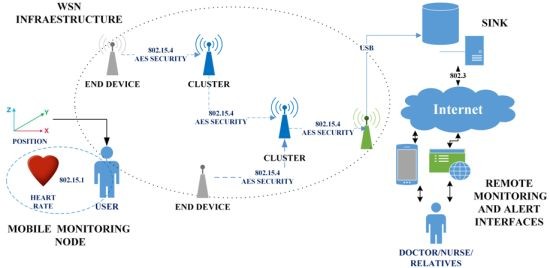
\includegraphics[width=8.5cm]{cluster}
\subsection{Application of WSN in Healthcare Monitoring}
\begin{flushleft}
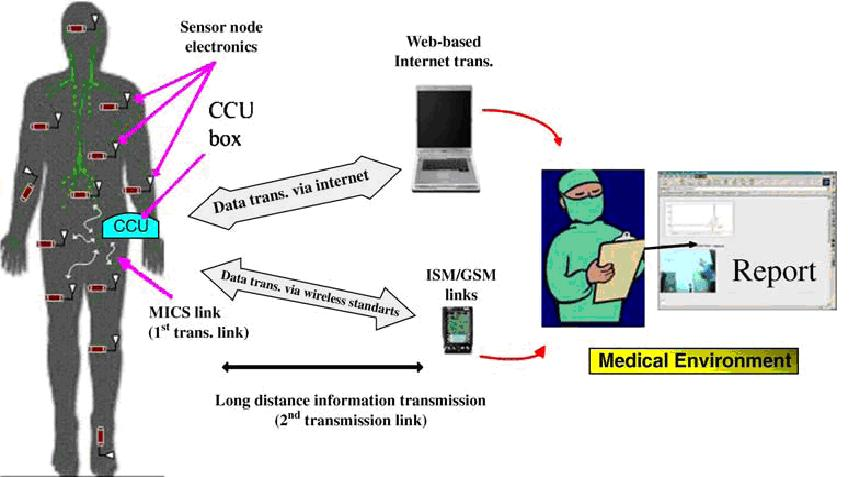
\includegraphics[width=8.5cm]{WSN}
\begin{itemize}
  \item Telemonitoring of Human Physiological Data
  \item Tracking and Monitoring Doctors and Patients inside a Hospital
  \item Drug Administration in Hospital
\end{itemize}
\end{flushleft}

\section{Cryptography Overview}
\begin{flushleft}
Cryptography is the practice and study of techniques for secure communication in presence of third parties called adversaries.
\linebreak
There are five functions of cryptography which must be followed by any algorithms used for cryptography.
\begin{itemize}
  \item Confidentiality
  \item Authentication
  \item Integrity
  \item Non-repudiation
  \item Key Exchange
\end{itemize}
\end{flushleft}

\subsection{Symmetric Key Cryptography}
\begin{flushleft}
In this type of cryptographic schemes same key is used for both encryption of plaintext and the description of ciphertext. The keys can be identical but some simple transformation is possible to go betweeen the keys. The keys must be shared before any transaction of messages can take place.
\linebreak

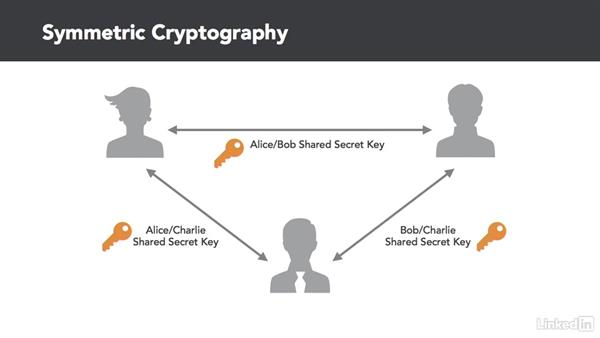
\includegraphics[width=8.5cm]{symmetric}
\end{flushleft}


\subsubsection{Deffie Hellman Key Sharing Algorithm}
\begin{flushleft}
One of the most famous key sharing algorithm that was the base for asymmetric key encryption is the Deffie Hellman Key Sharing algorithm. This algorithm ensures that the key is not compromised with any other malicious user.
\linebreak

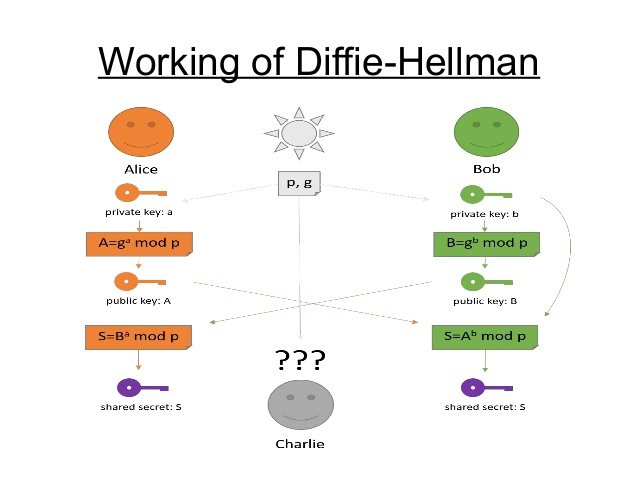
\includegraphics[width=8.5cm]{hellman}
\end{flushleft}


\subsubsection{AES Encryption}
\begin{flushleft}
AES is an Encryption algorithm based on substituition permutation network, and unlike DES it is not a algorithms based on Feistel Network. It is a variant of Rijindael which has a fixed block size 128 bits and a key size of 128, 192 and 	256 bits.
\linebreak
The security of AES encryption completely depends upon the length of the key and it is not breakable even if the algorithm is known. As we now that this encryption is breakable only by brute force attack to find out the key being used but considering the number of bits that is not a possibility because it is next to impossible to find out the key for which we have to find \(2^{192}\) combinations.
\begin{itemize}
  \item The keys for each round is derived from the cipher key, which was originally described in Rijindael's key schedule. The keys required are different for each round and it also have one more extra key for the initial round.
  \item Initial Round: Each byte of the state is combined with a block of the round key using bitwise xor.
  \item Then we have Rounds. In each round there are some steps which are required to be followed which includes
  \begin{itemize}
  \item SubBytes - each byte is replaced with another according to the Substitution Matrix.
  \item ShiftRows - Last three rows of the state are shifted cyclically.
  \item MixColumns - 4 bytes are combined in each column also called mixing.
  \item AddRoundKey
  \end{itemize}
  \item FinalRound which is same as the above round but no mixing takes place.
\end{itemize}

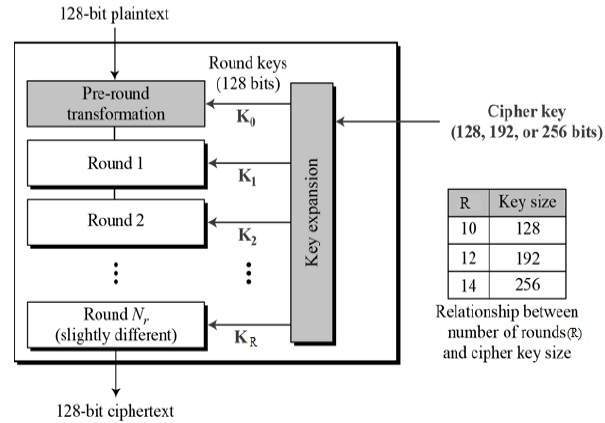
\includegraphics[width=8.5cm]{aes_structure}
\end{flushleft}

\subsection{Asymmetric Key Cryptography}
\begin{flushleft}
In this type of cryptographic scheme there are two different keys one called private key which is in the possesion of the individual and second one is called public key which is shared between all the people. One can send the encrypted message by encrypting the message with the help of public key and only the individual owning the key can decrypt the message.
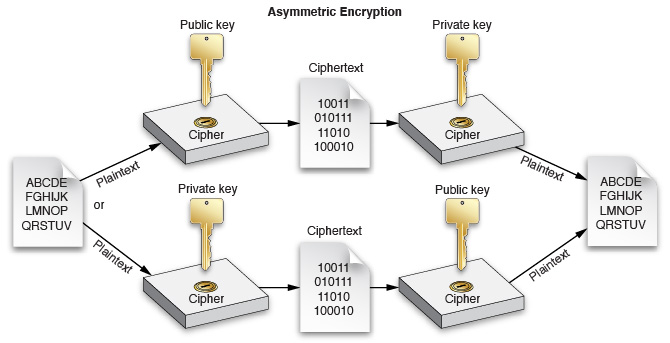
\includegraphics[width=8.5cm]{asymmetric}

\end{flushleft}

\subsubsection{RSA Encryption Scheme}
\begin{flushleft}
RSA is the most practical public key encryption algorithm and is used widely in transmission. This encryption is based on the difficulty of factorisation of the product of two large prime numbers.

The following steps shows the use of RSA scheme:
\begin{itemize}
  \item Two large prime numbers p and q and we have \(n = pq \), and \(\phi(n) = (p-1)(q-1)\).
  \item e is such that \(1 < e < \phi(n)\), and let m be the message, we select d such that \(ed = 1 (mod n)\), where e is the public key and d the private key.
  \item So \(E(m) = me  (mod\ n), D(E(m)) = med (mod\ n) = m (mod\ n)\) which is the original message
\end{itemize}

\end{flushleft}

\subsection{Energy Consumption of the above mentioned algorithms}
\begin{flushleft}
The encryption algorithms that are being used in present day encryption strategies have been discussed. The above encryption algorithm shows that it is not possible to break them easily(we can only use brute force to find the key) and provides one the factor of security but what about the other problem that we are facing, the time complexity, the energy consumption etc. An analysis done on the energy consumed in each algorithm is done with a 25MHz clocked processor and it's energy consumed values have been found out.
\end{flushleft}

\subsubsection{Energy Consumption in AES Scheme}
The amount of Energy used by AES Encryption scheme is shown in the fig. below. As it can be seen that the calculations are done using various block cipher schemes like ECB, CBC, so the power consumption also depends on the type of block cipher being used.
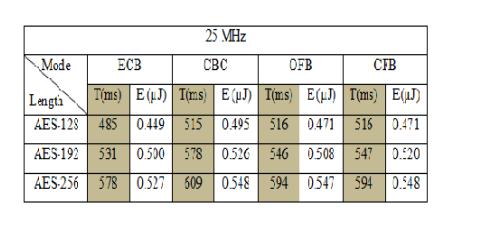
\includegraphics[width=8.5cm]{energy_aes}

\subsubsection{Energy Consumption in RSA Scheme}
The amount of Energy used by RSA Encryption scheme is shown in the fig. below. As we can infer that the time and energy consumed by RSA is quite greater than that of AES Scheme, so using RSA in WSN devices is not possible. The complexity is due to the selection of two prime factors and finding out their product. As the numbers are quite big, the energy consumed by them also increases.
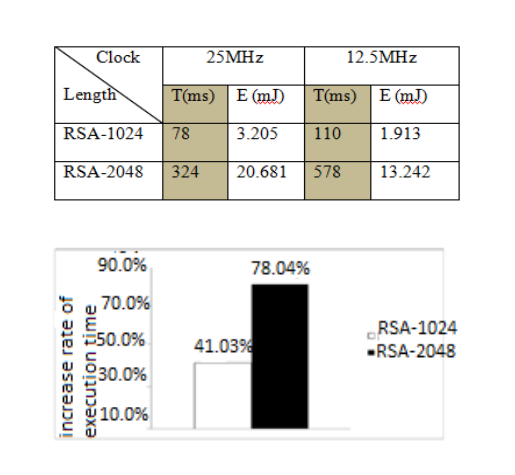
\includegraphics[width=8.5cm]{energy_rsa}
\section{LightWeight Cryptography Schemes for Energy Effecient Encryption in WSN}
\begin{flushleft}
We have seen that the RSA and AES uses a lot of energy and the battery life cannot be preserved for long if we are using them, so now some new schemes used in IoT is being introduced here. These algorithms has been made to reduce the energy consumptions and taking care of problems being faced regarding security in WSN.
\linebreak
Over the decade a lot of block ciphers, hash functions, message authentication codes, stream ciphers has been proposed for improved performance of already defined cryptographic standards. These Encryption are based on the fact that the attacker will have some constrains and that's why under the given conditions of IOT will not be able to crack encrypted code. The idea of light weight encryption is to utilize the conditions and have a better performance by maintaing a balance between security, performance and resource requirement.
\end{flushleft}

\subsection{LightWeight Block Ciphers}
LightWeight block ciphers uses lightweight designs and achieves advantages over conventional schemes. Some of the techniques used are
\begin{itemize}
  \item Smaller block sizes - To save memory
  \item Smaller key sizes - To save energy and computation time.
  \item Simpler Rounds - Less number of S-boxes as compared to AES.
  \item Simpler Key Schedules - Using Secure Key Derivation can prevent attacks.
  \item Minimal Implementation - Use of only one function at a device location.
\end{itemize}

\subsection{LightWeight Message Authentication Code}
A Messgae Authentication Code (MAC) generate a tag from message and a secret key, and is used to verify the authenticity and integrity of the message.

\subsection{LightWeight Stream Ciphers}
Generally Stream ciphers are not preferred to be used in non-constrained environment cause they are easy to crack compared to their alternatives block ciphers, but these stream ciphers can be utilised in LightWight Encryptions. Grain is widely analyzed algorithm involving stream cipher.

\section{Conclusion}
\begin{flushleft}
Security concerns constitute a potential stumbling block on the development of sensor Networks. The salient features of WSNs makes it hard to design the encryption algorithm and also designing strong security protocols. The Energy consumed by the famous and secure encryption algorithm is too high, and decreases the battery life by a huge factor. Different encryption algorithm schemes are provided like LightWeight Encryption Algorithms which are specifically made to reduce the energy consumption. Due to the advancement in WSN, the cryptographic schemes being proposed now are considering time as well as energy trade off which increases the complexity in algorithm design.
\end{flushleft}

\ifCLASSOPTIONcaptionsoff
  \newpage
\fi

\begin{thebibliography}{1}

\bibitem{SWBS}
Geoff Appleboom, Elvis Camacho, Mickey E Abraham\emph{"Smart wearable body sensors for patient self-assessment and monitoring"}, \hskip 1em plus
  0.5em minus 0.4em\relax BioMed Central.

\bibitem{WSNKeyManagement}
Ju-Hyung Son, Jun-Sik Lee, Seung-Woo Seo \emph{"Energy Efficient Group Key Management Scheme for Wireless Sensor Networks"}, \hskip 1em plus
  0.5em minus 0.4em\relax IEEE Xplorer, July 2007.
  
\bibitem{WSNKeyAAgreement}
Thomas R. Halford, Keith M. Chugg \emph{"Energy Efficient Group Key Agreement for Wireless Networks"}, \hskip 1em plus
  0.5em minus 0.4em\relax IEEE Xplorer, August 2015.
  
\bibitem{WSNAdHoc}
Thomas R. Halford, Thomas A. Cortade, Keith M. Chugg \emph{"Energy Efficient Secure Group Key agreement for ad hoc networks"}, \hskip 1em plus
  0.5em minus 0.4em\relax IEEE Xplorer, December 2013.
  
\bibitem{DCEER}
T. T. Huynh and T. N. Tran and C. H. Tran and A. V. Dinh-Duc \emph{"Delay constraint energy-efficient routing based on Lagrange relaxation in wireless sensor networks"}, \hskip 1em plus
  0.5em minus 0.4em\relax IEEE Xplorer, September 2017.
  
\bibitem{FPO}
J. Li, X. Hou, D. Su and J. D. D. Munyemana \emph{"Fuzzy power-optimised clustering routing algorithm for wireless sensor networks"}, \hskip 1em plus
  0.5em minus 0.4em\relax IEEE Xplorer, September 2017.
  
\bibitem{WSNHM}
Ashraf Darwish, Aboul Ella Hassanien \emph{"Wearable and Implantable Wireless Sensor Network Solutions for Healthcare Monitoring"},\hskip 1em plus
  0.5em minus 0.4em\relax Sensor Bessel, July 2012.

\bibitem{AIS}
\url{https//en.wikipedia.org/wiki/Artificial_immune_system}, Artificial Immune System

\bibitem{HHMSWSN}
Media Aminian, Hamid Reza Naji \emph{"A Hospital Healthcare Monitoring System Using Wireless Sensor Networks"},\hskip 1em plus
  0.5em minus 0.4em\relax Journal of Health and Medical Informatics, Februrary 2013.

\bibitem{LightWeightCrypto}
\url{http://nvlpubs.nist.gov/nistpubs/ir/2017/NIST.IR.8114.pdf}, LightWeight Cryptography
\end{thebibliography}

\end{document}


